\documentclass[12pt]{report} % You can use 'article' or 'book' class as well

\usepackage{graphicx} % For including images
\usepackage{amsmath}
\usepackage{amssymb}
\usepackage{caption}
\usepackage{hyperref}
\usepackage{multicol}
\usepackage{pgfplots}
\usepackage{tikz}
\usepgfplotslibrary{fillbetween}
\pgfplotsset{compat=1.18}

\begin{document}

% Title page
\begin{titlepage}
	\centering
	\vspace*{1cm} % Adjusts vertical space for the image
	% Insert your image (use the actual path and filename of your image)
	\includegraphics[width=0.3\textwidth]{../images/KMITL Logo.png} % Adjust width as needed

	\vspace{1cm} % Vertical space after the image
	{\LARGE \textbf{Week 11 Homework}} \\[0.5cm] % Title
	\vspace{0.5cm}
	{\large \textbf{Probability Model and Data Analysis}} \\[0.5cm]
    {\large \textbf{Software Engineering Program,}} \\[0.5cm]
	{\large \textbf{Department of Computer Engineering,}} \\[0.5cm]
	{\large \textbf{School of Engineering, KMITL}} \\[1cm]
    {\Large 67011352 Theepakorn Phayonrat} \\[0.5cm] % Authors (Use \\ the separate authors)
\end{titlepage}

\section*{Homework of Continuous RVs}

\subsection*{Question}

\noindent Continuous random variable $X$ has $E[X] = 3$ and
$Var[X] = 9$. Find the PDF, $f_{X}(x)$, if \\

\noindent (a) $X$ is an exponential random variable, \\
\noindent (b) $X$ is a continuous uniform random variable. \\

\subsection*{Solution}

\noindent (a) \\

We know that, $E[X] = 3$ and $Var[X] = 9$. \\

\begin{align*}
    E[X] & = \frac{1}{\lambda} \\
    \frac{1}{\lambda} & = 3 \\
    \therefore \lambda & = \frac{1}{3} \\
\end{align*}

\[
    \therefore f_{X}(x) =
    \begin{cases}
        \dfrac{e^{-\frac{x}{3}}}{3} & x \ge 0 \\
        0 & otherwise
    \end{cases}
\]

\newpage

\noindent (b) \\

We know that, $E[X] = 3$

\begin{align*}
    E[X] & = \frac{(b + a)}{2} \\
    \frac{(b + a)}{2} & = 3 \\
    \therefore b + a & = 6 \tag{1} \\
\end{align*}

We know that, $Var[X] = 9$

\begin{align*}
    V[X] & = \frac{(b - a)^{2}}{12} \\
    \frac{(b - a)^{2}}{12} & = 9 \\
    (b - a)^{2} & = 108 \\
    b - a & = \sqrt{108} = 6\sqrt{3} \tag{2} \\
\end{align*}

(1) + (2) \\

\begin{align*}
    (b + a) + (b - a) & = 6 + 6\sqrt{3} \\
    2b & = 2(3 + 3\sqrt{3}) \\
    \therefore b & = 3 + 3\sqrt{3} \\
    \therefore a & = 6 - b = 6 - (3 + 3\sqrt{3}) = 3 - 3\sqrt{3} \\
\end{align}

\[
    \therefore f_{X}(x) =
    \begin{cases}
        \dfrac{1}{6\sqrt{3}} & (3 - 3\sqrt{3}) \le x \le (3 + 3\sqrt{3}) \\
        0 & otherwise
    \end{cases}
\]

\newpage

\section*{Homework of Gaussian-RV}

\subsection*{Question 1}

\noindent $X$ is the Gaussian (0, 1) random variable and $Y$ is the Gaussian (0, 2) random variable. \\

\noindent (1) Sketch the PDFs $f_{X}(x)$ and $f_{Y}(y)$ in the same axes. \\
\noindent (2) What is $P[-1 < X \le 1]$? \\
\noindent (3) What is $P[-1 < Y \le 1]$? \\
\noindent (4) What is $P[X > 3.5]$? \\
\noindent (5) What is $P[Y > 3.5]$?

\subsection*{Solution}

\noindent (1) \\

\indent From the information provided earlier we can find the $f_{X}(x)$.

\begin{align*}
    f_{X}(x) & = \frac{1}{\sqrt{2\pi\sigma_{x}^{2}}}e^\frac{{-(x - \mu_{x})^{2}}}{2\sigma_{x}^{2}} \\
             & = \frac{1}{\sqrt{2\pi1^{2}}}e^\frac{{-(x - 0)^{2}}}{2(1)^{2}} \\
    \therefore  f_{X}(x) & = \frac{1}{\sqrt{2\pi}}e^\frac{{-x^{2}}}{2} \\
\end{align*}

Now we can sketch the graph of $f_{X}(x)$.

\begin{figure}[h!]
    \centering
    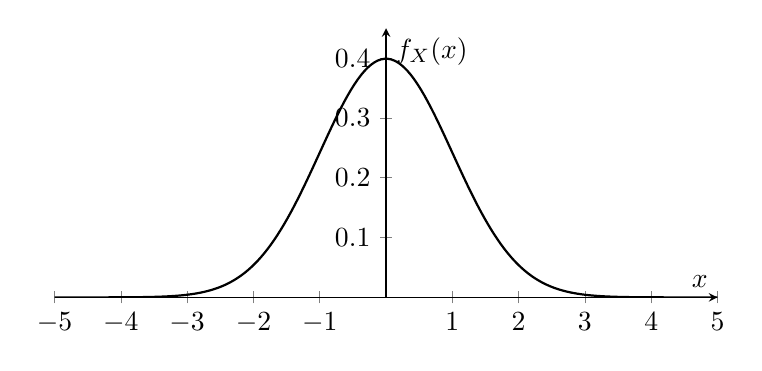
\begin{tikzpicture}
        \begin{axis}[
            domain=-5:5, 
            ymin=0,
            ymax=0.45,
            samples=200,
            axis lines=middle,
            xlabel={$x$},
            ylabel={$f_{X}(x)$},
            width=10cm,
            height=5cm,
            ytick distance=0.1,
            xtick distance=1,
            yticklabel={\pgfmathprintnumber[fixed, precision=2]{\tick}}
        ]
        ]
        \addplot[thick] {1/(sqrt(2*pi)) * exp(-x^2/(2))};
        \end{axis}
    \end{tikzpicture}
\end{figure}

\newpage

\indent From the information provided earlier we can find the $f_{Y}(y)$.

\begin{align*}
    f_{Y}(y) & = \frac{1}{\sqrt{2\pi\sigma_{y}^{2}}}e^\frac{{-(y - \mu_{y})^{2}}}{2\sigma_{y}^{2}} \\
    & = \frac{1}{\sqrt{2\pi2^{2}}}e^\frac{{-(y - 0)^{2}}}{2(2)^{2}} \\
    \therefore f_{Y}(y) & = \frac{1}{\sqrt{8\pi}}e^\frac{-y^{2}}{8} \\
\end{align*}

Now we can sketch the graph of $f_{Y}(y)$.

\begin{figure}[h!]
    \centering
    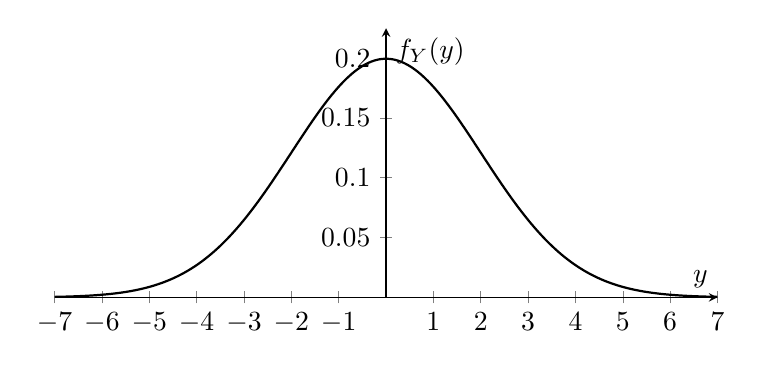
\begin{tikzpicture}
        \begin{axis}[
            domain=-7:7, 
            ymin=0,
            ymax=0.225,
            samples=200,
            axis lines=middle,
            xlabel={$y$},
            ylabel={$f_{Y}(y)$},
            width=10cm,
            height=5cm,
            ytick distance=0.05,
            xtick distance=1,
            yticklabel={\pgfmathprintnumber[fixed, precision=2]{\tick}}
        ]
        \addplot[thick] {1/(sqrt(8*pi)) * exp(-x^2/(8))};
        \end{axis}
    \end{tikzpicture}
\end{figure}

\newpage

\subsection*{Positive Z Table}

\includegraphics[width=\textwidth]{./image/positiveztable.png}

Source: \url{https://www.ztable.net/}

\newpage

\noindent (2) \\

\begin{figure}[h!]
    \centering
    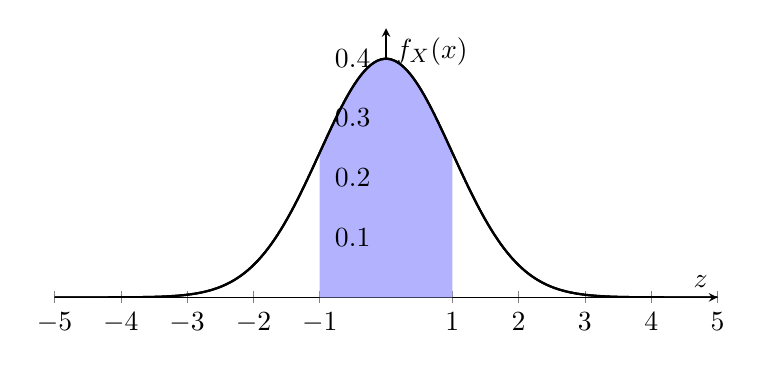
\begin{tikzpicture}
        \begin{axis}[
            domain=-5:5, 
            ymin=0,
            ymax=0.45,
            samples=200,
            axis lines=middle,
            xlabel={$z$},
            ylabel={$f_{X}(x)$},
            width=10cm,
            height=5cm,
            ytick distance=0.1,
            xtick distance=1,
            yticklabel={\pgfmathprintnumber[fixed, precision=2]{\tick}}
        ]
        \addplot[thick] {1/(sqrt(2*pi)) * exp(-x^2/(2))};
        % Define the PDF
        \addplot[thick, name path=curve] {1/(sqrt(2*pi)) * exp(-x^2/(2))};

        % Define x-axis for filling
        \path[name path=axis] (axis cs:-7,0) -- (axis cs:7,0);

        % Shade between -1 and 1
        \addplot[
            thick,
            color=blue!50,
            fill=blue!30,
        ]
        fill between[
            of=curve and axis,
            soft clip={domain=-1:1},
        ];
        \end{axis}
    \end{tikzpicture}
\end{figure}

\begin{align*}
    P[-1 \le X \le 1] & = \Phi(z_{2}) - \Phi(z_{1}) \\
    & = \Phi(\frac{x_{2} - \mu_{x}}{\sigma_{x}}) - \Phi(\frac{x_{1} - \mu_{x}}{\sigma_{x}}) \\
    & = \Phi(\frac{1 - 0}{1}) - \Phi(\frac{-1 - 0}{1}) \\
    & = \Phi(1) - \Phi(-1) \\
    & = \Phi(1) - (1 - \Phi(1)) \\
    & = 2\Phi(1) - 1 \\
    & = 2(0.8413) - 1 \\
    \therefore P[-1 \le X \le 1]& = 1.6826 - 1 = 0.6826 \\
\end{align*}

\newpage

\noindent (3)

\begin{figure}[h!]
    \centering
    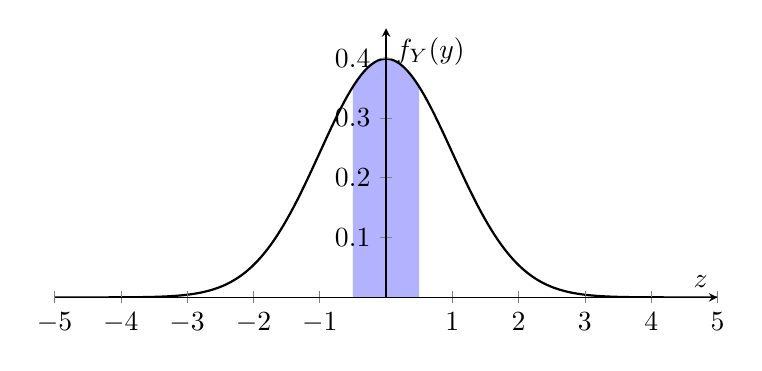
\begin{tikzpicture}
        \begin{axis}[
            domain=-5:5, 
            ymin=0,
            ymax=0.45,
            samples=200,
            axis lines=middle,
            axis on top,
            xlabel={$z$},
            ylabel={$f_{Y}(y)$},
            width=10cm,
            height=5cm,
            ytick distance=0.1,
            xtick distance=1,
            yticklabel={\pgfmathprintnumber[fixed, precision=2]{\tick}}
        ]
        % Define the PDF
        \addplot[thick, name path=curve] {1/(sqrt(2*pi)) * exp(-x^2/(2))};

        % Define x-axis for filling
        \path[name path=axis] (axis cs:-7,0) -- (axis cs:7,0);

        % Shade between -1 and 1
        \addplot[
            thick,
            color=blue!50,
            fill=blue!30,
        ]
        fill between[
            of=curve and axis,
            soft clip={domain=-0.5:0.5},
        ];
        \end{axis}
    \end{tikzpicture}
\end{figure}

\begin{align*}
    P[-1 \le Y \le 1] & = \Phi(z_{2}) - \Phi(z_{1}) \\
    & = \Phi(\frac{y_{2} - \mu_{y}}{\sigma_{y}}) - \Phi(\frac{y_{1} - \mu_{y}}{\sigma_{y}}) \\
    & = \Phi(\frac{1 - 0}{2}) - \Phi(\frac{-1 - 0}{2}) \\
    & = \Phi(\frac{1}{2}) - \Phi(-\frac{1}{2}) \\
    & = \Phi(0.5) - (1 - \Phi(0.5)) \\
    & = 2\Phi(0.5) - 1 \\
    & = 2(0.6915) - 1 \\
    \therefore P[-1 \le Y \le 1]& = 1.3830- 1 = 0.3830 \\
\end{align*}

\newpage

\noindent (4)

\begin{figure}[h!]
    \centering
    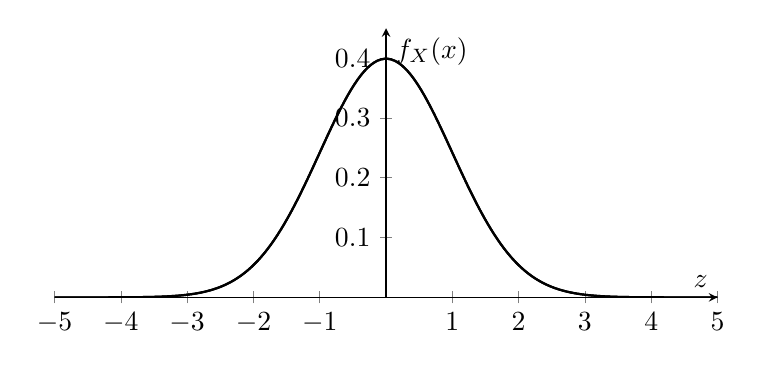
\begin{tikzpicture}
        \begin{axis}[
            domain=-5:5, 
            ymin=0,
            ymax=0.45,
            samples=200,
            axis lines=middle,
            xlabel={$z$},
            ylabel={$f_{X}(x)$},
            width=10cm,
            height=5cm,
            ytick distance=0.1,
            xtick distance=1,
            yticklabel={\pgfmathprintnumber[fixed, precision=2]{\tick}}
        ]
        \addplot[thick] {1/(sqrt(2*pi)) * exp(-x^2/(2))};
        % Define the PDF
        \addplot[thick, name path=curve] {1/(sqrt(2*pi)) * exp(-x^2/(2))};

        % Define x-axis for filling
        \path[name path=axis] (axis cs:-7,0) -- (axis cs:7,0);

        % Shade between -1 and 1
        \addplot[
            thick,
            color=blue!50,
            fill=blue!30,
        ]
        fill between[
            of=curve and axis,
            soft clip={domain=3.5:5},
        ];
        \end{axis}
    \end{tikzpicture}
    \captionsetup{labelformat=empty}
    \caption{The highlight is very small because its boundary is [3.5, \infty)}
\end{figure}

\begin{align*}
    P[X \ge 3.5] & = \Phi(z_{2}) - \Phi(z_{1}) \\
    & = \Phi(\frac{x_{2} - \mu_{x}}{\sigma_{x}}) - \Phi(\frac{x_{1} - \mu_{x}}{\sigma_{x}}) \\
    & = \Phi(\frac{\infty - 0}{1}) - \Phi(\frac{3.5 - 0}{1}) \\
    & = \Phi(\infty) - \Phi(3.5) \\
    \therefore P[X \ge 3.5]& = 1 - 0.99977 \approx 0.00023 =  2.3 \times 10^{-4} \\
\end{align*}

\newpage

\noindent (5)

\begin{figure}[h!]
    \centering
    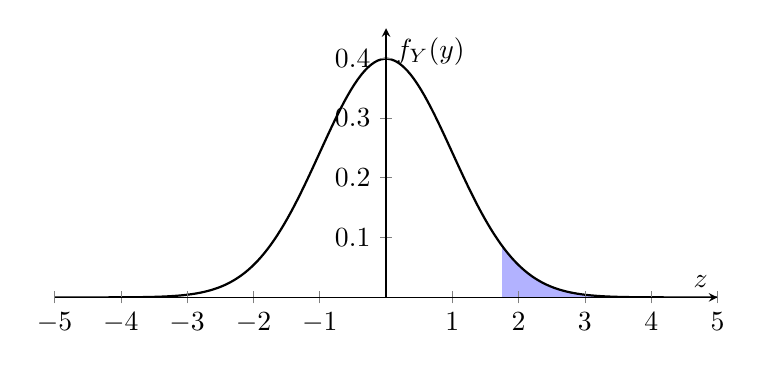
\begin{tikzpicture}
        \begin{axis}[
            domain=-5:5, 
            ymin=0,
            ymax=0.45,
            samples=200,
            axis lines=middle,
            axis on top,
            xlabel={$z$},
            ylabel={$f_{Y}(y)$},
            width=10cm,
            height=5cm,
            ytick distance=0.1,
            xtick distance=1,
            yticklabel={\pgfmathprintnumber[fixed, precision=2]{\tick}}
        ]
        % Define the PDF
        \addplot[thick, name path=curve] {1/(sqrt(2*pi)) * exp(-x^2/(2))};

        % Define x-axis for filling
        \path[name path=axis] (axis cs:-7,0) -- (axis cs:7,0);

        % Shade between -1 and 1
        \addplot[
            thick,
            color=blue!50,
            fill=blue!30,
        ]
        fill between[
            of=curve and axis,
            soft clip={domain=1.75:7},
        ];
        \end{axis}
    \end{tikzpicture}
\end{figure}

\begin{align*}
    P[Y \ge 3.5] & = \Phi(z_{2}) - \Phi(z_{1}) \\
    & = \Phi(\frac{y_{2} - \mu_{y}}{\sigma_{y}}) - \Phi(\frac{y_{1} - \mu_{y}}{\sigma_{y}}) \\
    & = \Phi(\frac{\infty - 0}{2}) - \Phi(\frac{3.5 - 0}{2}) \\
    & = \Phi(\infty) - \Phi(1.75) \\
    & = 1 - 0.95994 \\
    \therefore P[Y \ge 3.5]& \approx 0.04006 \\
\end{align*}

\newpage

\subsection*{Question 2}

\noindent The peak temperature $T$, in degrees Fahrenheit, on a July
day in Antarctica is a Gaussian random variable with a variance of 225.
With probability $\frac{1}{2}$, the temperature $T$ exceeds 10 degrees.

\noindent (1) What is $P[T > 32]$, the probability the temperature is
above freezing? \\
\noindent (2) What is $P[T < 0]$? \\
\noindent (3) What is $P[T > 60]$? \\

\subsection*{Solution}

From the information provided from earlier, we know that, $Var[T] = 225$
and $P[T \ge 10] = \frac{1}{2}$. \\

\begin{align*}
    \sigma_{T} & = \sqrt{Var[T]} \\
    & = \sqrt{225} \\
    \therefore \sigma_{T} & = 15 \\
\end{align*}

\begin{align*}
    P[T > 10] & = \Phi(\frac{\infty - \mu_{T}}{\sigma_{T}}) - \Phi(\frac{t - \mu_{T}}{\sigma_{T}}) \\
    \frac{1}{2} & = \Phi(\infty) - \Phi(\frac{t -\mu_{T}}{15}) \\
    \frac{1}{2} & = 1 - \Phi(\frac{10 -\mu_{T}}{15}) \\
    \Phi(\frac{10 -\mu_{T}}{15}) & = \frac{1}{2} \\
    \Phi(\frac{10 -\mu_{T}}{15}) & = \Phi(0) \\
    \therefore \mu_{T} & = 10 \\
\end{align*}

\newpage

\noindent (1)

\begin{figure}[h!]
    \centering
    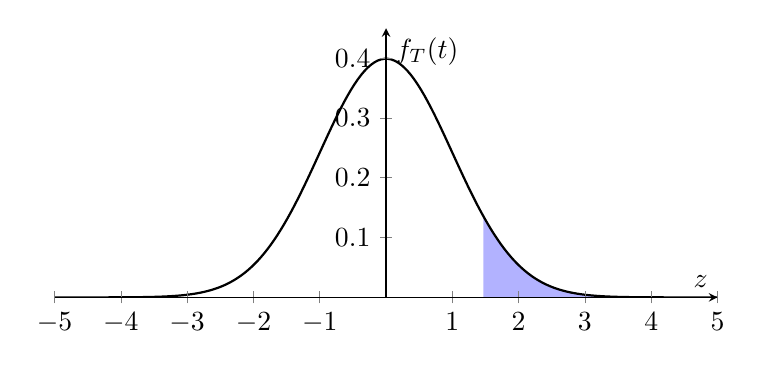
\begin{tikzpicture}
        \begin{axis}[
            domain=-5:5, 
            ymin=0,
            ymax=0.45,
            samples=200,
            axis lines=middle,
            axis on top,
            xlabel={$z$},
            ylabel={$f_{T}(t)$},
            width=10cm,
            height=5cm,
            ytick distance=0.1,
            xtick distance=1,
            yticklabel={\pgfmathprintnumber[fixed, precision=2]{\tick}}
        ]
        % Define the PDF
        \addplot[thick, name path=curve] {1/(sqrt(2*pi)) * exp(-x^2/(2))};

        % Define x-axis for filling
        \path[name path=axis] (axis cs:-7,0) -- (axis cs:7,0);

        % Shade between -1 and 1
        \addplot[
            thick,
            color=blue!50,
            fill=blue!30,
        ]
        fill between[
            of=curve and axis,
            soft clip={domain=1.467:7},
        ];
        \end{axis}
    \end{tikzpicture}
\end{figure}

\begin{align*}
    P[T > 32] & = \Phi(z_{2}) - \Phi(z_{1}) \\
    & = \Phi(\frac{t_{2} - \mu_{T}}{\sigma_{T}}) - \Phi(\frac{t_{1} - \mu_{T}}{\sigma_{T}}) \\
    & = \Phi(\frac{\infty - 10}{15}) - \Phi(\frac{32 - 10}{15}) \\
    & = \Phi(\infty) - \Phi(\frac{22}{15}) \\
    & = \Phi(\infty) - \Phi(1.47) \\
    & = 1 - 0.92922 \\
    \therefore P[T > 32]& \approx 0.07078 \approx 0.0708 \\
\end{align*}

\newpage

\noindent (2)

\begin{figure}[h!]
    \centering
    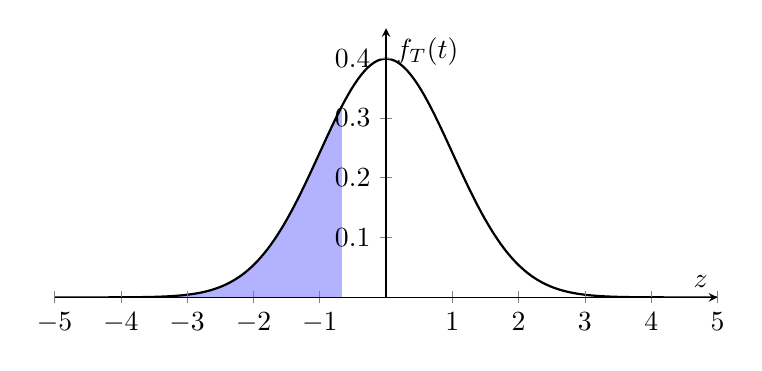
\begin{tikzpicture}
        \begin{axis}[
            domain=-5:5, 
            ymin=0,
            ymax=0.45,
            samples=200,
            axis lines=middle,
            axis on top,
            xlabel={$z$},
            ylabel={$f_{T}(t)$},
            width=10cm,
            height=5cm,
            ytick distance=0.1,
            xtick distance=1,
            yticklabel={\pgfmathprintnumber[fixed, precision=2]{\tick}}
        ]
        % Define the PDF
        \addplot[thick, name path=curve] {1/(sqrt(2*pi)) * exp(-x^2/(2))};

        % Define x-axis for filling
        \path[name path=axis] (axis cs:-7,0) -- (axis cs:7,0);

        % Shade between -1 and 1
        \addplot[
            thick,
            color=blue!50,
            fill=blue!30,
        ]
        fill between[
            of=curve and axis,
            soft clip={domain=-7:-0.667},
        ];
        \end{axis}
    \end{tikzpicture}
\end{figure}

\begin{align*}
    P[T < 0] & = \Phi(z_{2}) - \Phi(z_{1}) \\
    & = \Phi(\frac{t_{2} - \mu_{T}}{\sigma_{T}}) - \Phi(\frac{t_{1} - \mu_{T}}{\sigma_{T}}) \\
    & = \Phi(\frac{0 - 10}{15}) - \Phi(\frac{-\infty - 10}{15}) \\
    & = \Phi(-\frac{2}{3}) - \Phi(-\infty) \\
    & = \Phi(-0.667) - \Phi(-\infty) \\
    & = (1 - \Phi(0.67)) - \Phi(-\infty) \\
    & = (1 - 0.74857) - 0 \\
    \therefore P[T < 0]& \approx 0.25143 \approx 0.2514 \\
\end{align*}

\newpage

\noindent (3)

\begin{figure}[h!]
    \centering
    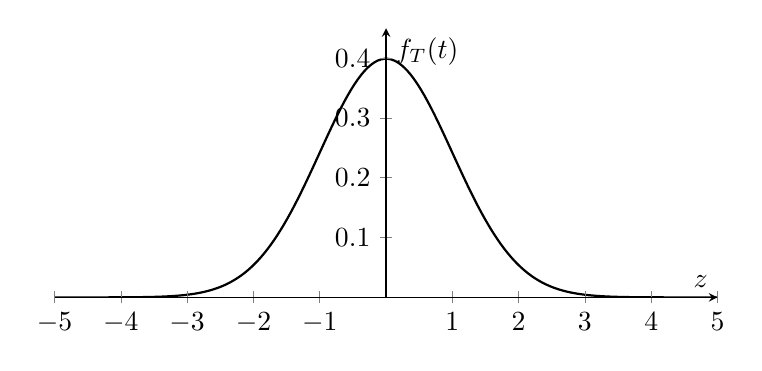
\begin{tikzpicture}
        \begin{axis}[
            domain=-5:5, 
            ymin=0,
            ymax=0.45,
            samples=200,
            axis lines=middle,
            axis on top,
            xlabel={$z$},
            ylabel={$f_{T}(t)$},
            width=10cm,
            height=5cm,
            ytick distance=0.1,
            xtick distance=1,
            yticklabel={\pgfmathprintnumber[fixed, precision=2]{\tick}}
        ]
        % Define the PDF
        \addplot[thick, name path=curve] {1/(sqrt(2*pi)) * exp(-x^2/(2))};

        % Define x-axis for filling
        \path[name path=axis] (axis cs:-7,0) -- (axis cs:7,0);

        % Shade between -1 and 1
        \addplot[
            thick,
            color=blue!50,
            fill=blue!30,
        ]
        fill between[
            of=curve and axis,
            soft clip={domain=3.33:7},
        ];
        \end{axis}
    \end{tikzpicture}
    \captionsetup{labelformat=empty}
    \caption{The highlight is very small because its boundary is [3.33, \infty)}
\end{figure}

\begin{align*}
    P[T > 60] & = \Phi(z_{2}) - \Phi(z_{1}) \\
    & = \Phi(\frac{t_{2} - \mu_{T}}{\sigma_{T}}) - \Phi(\frac{t_{1} - \mu_{T}}{\sigma_{T}}) \\
    & = \Phi(\frac{0\infty - 10}{15}) - \Phi(\frac{60 - 10}{15}) \\
    & = \Phi(\infty) - \Phi(\frac{50}{15}) \\
    & = \Phi(\infty) - \Phi(\frac{10}{3}) \\
    & = \Phi(\infty) - \Phi(3.33) \\
    & = 1 - 0.99957 \\
    \therefore P[T > 60]& \approx 0.00043 = 4.3 \times 10^{-4}\\
\end{align*}

\end{document}
